% Use class option [extendedabs] to prepare the 1-page extended abstract.
\documentclass[extendedabs]{bmvc2k}
\usepackage[colorlinks = true,
            linkcolor = blue,
            urlcolor  = blue,
            citecolor = blue,
            anchorcolor = blue]{hyperref}
\usepackage{kotex}
% for the fancy \koTeX logo
\usepackage{kotex-logo}

% Document starts here
\begin{document}


\title{VGGNet \& ResNet pre-report}
\addauthor{
김태훈$^{1}$
}{}{1}

\addinstitution{
$^1$부산대학교 전기컴퓨터공학부.  
}

 
\maketitle
\noindent

\begin{figure}[t]
	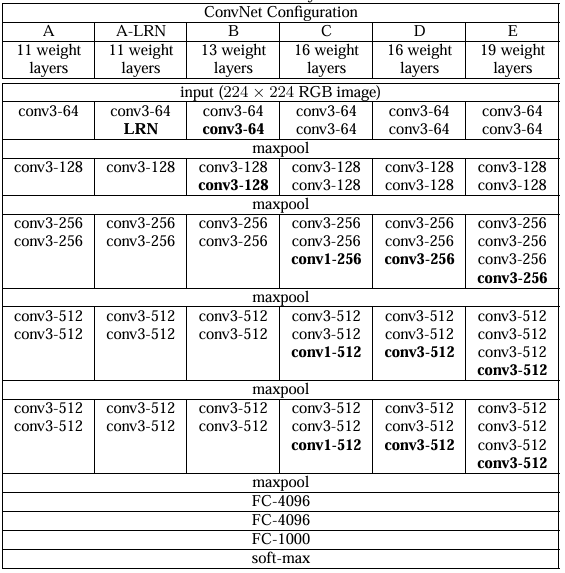
\includegraphics[width=\linewidth]{images/vggnet.PNG}
	\caption{VGGNet paper\cite{simonyan2015deepconvolutionalnetworkslargescale} 에서 실험한 ConvNet 구조. (A)에서 (E)로 갈수록 깊이가 깊어진다(layer가 추가되며, 추가된 layer는 굵게 표시됨.). Convolution layer의 파라미터는 conv<필터 크기>-<채널 개수>로 표시된다.}
 \label{fig:VGGNet}
	\vspace{-2mm}
\end{figure}
\section{VGGNet}
VGGNet\cite{simonyan2015deepconvolutionalnetworkslargescale}은 Deep ConvNet을 사용하여 ILSVRC-2012에서 우승한 Alex-Net\cite{AlexNet}에서 깊이를 늘려서(즉, 더 많은 Convolution layer를 추가하여) 정확도를 높인 ConvNet이다. 이것이 실행가능한 이유는 모든 layer가 $(3 \times 3)$ 의 필터 크기를 가지고 있기 때문이다.
\subsection{Architecture}
input의 크기는 $224 \times 224$ RGB 이미지이며, 이미지는 훈련 데이터의 평균 RGB 값을 각 이미지에서 빼서 전처리한다. convolution layer는 $(3 \times 3)$ 의 필터 크기를 가지고 있다. 일부 $(1 \times 1)$ 필터도 있는데, 이는 이미지의 크기를 보존하면서 비선형성을 추가한다. stride는 1이며 padding은 convolution 연산 후 이미지 크기가 보존되도록 한다(즉, $(3 \times 3)$필터 크기에서 1). Max-pooling은 5개가 있으며, 그 사이에 convolution layer가 여러개 들어간다. Max-pooling은 $2\times 2$ 크기의 커널에 stride는 2이다. 즉 Max-pooling을 지난 후 이미지 크기는 반으로 줄어든다. 

모든 Convolution layer를 지난 후에는 3개의 Fully-Connected layer가 있으며, 처음 2개는 4096, 마지막 1개는 1000개의 퍼셉트론을 가진다. layer와 layer 사이에는 ReLU\cite{AlexNet} 비선형 함수가 적용되어있으며, 마지막 Fully-Connected layer 이후에는 softmax가 적용되어 있다.

\cite{simonyan2015deepconvolutionalnetworkslargescale}에서 구성한 6개의 신경망 구조가 \ref{fig:VGGNet}에 나와있다. A(11 layers)에서 E(19 layers)로 갈수록 깊이가 깊어지며, 구조는 앞서 설명한 것과 동일하다. Convolution layer의 채널 개수는 64개부터 시작하여 Max-Pooling을 지날때 마다 2배씩 증가한다.

필터 크기를 줄임으로서, 깊이가 깊어져도 학습해야할 가중치 개수는 깊이가 8인 \cite{overfeat}보다 크지 않다.
\subsection{Discussion}
VGGNet은 이전 Alexnet\cite{AlexNet} 등에서 사용한 ConvNet과 차이나는 부분은 첫 layer의 필터 크기이다. VGGNet에서 사용한 필터 크기는 $(3\times 3)$ 에 stride 1이며, Alexnet\cite{AlexNet}에서 사용한 필터 크기는 $(11\times 11)$에 stride 4이다.

2개의 $3 \times 3$ Convolution layer는 1개의 $5\times 5$ 역할을 할 수 있으며, 3개의 $3 \times 3$ Convolution layer는 1개의 $7\times 7$ 역할을 할 수 있다고 한다. 이때 채널 개수가 $C$개라고 할 때, 3개의$ 3\times 3$ Convolution layer는 $3(3^2C^2)=27C^2$ 가중치가 있는데 반해 1개의 $7\times 7$ Convolution layer는 $7^2C^2=49C^2$의 가중치를 가지고 있어 3개의$ 3\times 3$ Convolution layer가 더 효율적이다.

\subsection{Classification}
\subsubsection{Training}
ConvNet 훈련 과정에서, 배치 크기는 256, momentum은 0.9로 설정하였다고 한다. 또한 $L_2$정규화$(\lambda = 5\dots10^{-4})$를 적용하였으며 처음 두 Fully Connected layer에 dropout(ratio=0.5)를 적용하였다고 한다. 학습률은 0.01로 설정되었고, validation set의 정확도가 오르지 않을 때 마다 10배씩 학습률을 낮추었다고 한다.

훈련에 사용된 이미지는 2가지 방법을 적용하여 이미지 크기를 조정하였다. 첫번째 방법은 $(256\times256)$ 나 $(384\times384)$의 크기로 모든 사진을 같은 크기로 조정하는 것이다.

두번째 방법은 $[S_{min},S_{max}]$ 범위에서 무작위로 선택하여 이미지 크기를 조정하는 것이다. 이러한 방법을 scale-jittering이라 하며 이것을 통해 다양한 이미지 크기에 대해 정확도를 높일 수 있다. 학습 속도를 높이기 위해$(384\times384)$ 의 사진으로 학습한 모델에서 fine-tuning 한다.

이러한 방식으로 얻은 사진들을 $(224\times224)$의 크기로 무작위로 잘라서 사용한다(SGD iteration 마다 이미지 당 1개 씩 자름). 또한 자른 사진들은 무작위로 수평 뒤집기와 RGB color shift를 적용한다.

\subsubsection{Testing}
테스트에 사용한 이미지도 이미지 크기를 조정하였다. 조정된 이미지 크기는 \ref{fig:VGGNetSingleErr}을 참고한다.

테스트할 때 Fully-Connected layer를 convolution layer로 변환하였고, 최종 출력에서 채널 수가 분류해야할 클래스 수와 같게 하였다. 그리고 global average pooling을 적용하여 최종적으로 $1\times1000$의 출력이 되게 하였다.

\subsubsection{Performance}
single-scale test의 경우 \ref{fig:VGGNetSingleErr}와 같다. 깊이가 깊어질수록, scale-jittering을 사용하였을 때 결과가 좋다는 것을 확인할 수 있다. B net에 10개의 $3\times3$ convolution layer를 5개의 $5\times5$ convolution layer로 바꾸어서 실험하였을 때 top-1 error가 7\% 높게 나왔다고 하며, 작은 커널 크기로 구성된 깊은 convolution layer가 좋다는 것을 확인할 수 있다.

\begin{figure}[t]
	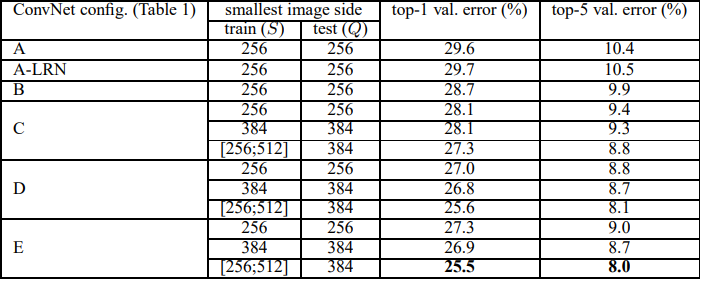
\includegraphics[width=\linewidth]{images/vggnet_single.PNG}
	\caption{단일 테스트 이미지 크기에서 성능}
 \label{fig:VGGNetSingleErr}
	\vspace{-2mm}
\end{figure}

\begin{figure}[t]
	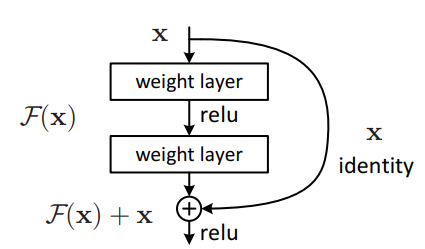
\includegraphics[width=\linewidth]{images/residual.PNG}
	\caption{Residual Learning}
 \label{fig:ResidualLearning}
	\vspace{-2mm}
\end{figure}

\section{ResNet}
ResNet\cite{resnet}은 \ref{fig:ResidualLearning}와 깉이 얕은 layer의 출력을 더 깊은 layer로 직접 전달하여 정확도를 높인 모델이다.

\subsection{Introduction}
\cite{simonyan2015deepconvolutionalnetworkslargescale} 등의 연구에서, 많은 layer를 가진 깊은 Convolution layer가 Imagenet Dataset Challenge에 효과적이라는 것을 확인했다. 그러나 layer가 많아질수록, 기울기 소실 또는 폭주가 발생한다. 즉 역전파 과정에서 출력 layer에서 먼 layer는 미분 연쇄 법칙에 의해 미분 결과값이 소실하거나, 또는 폭주하여 학습 초기부터 수렴하는 것을 방해한다. 이것을 해결하기 위해 Batch Normalization 등의 방법이 있다.

깊은 네트워크가 수렴할 때, degradation 문제, 즉 네트워크 깊이가 증가할 수록 정확도 증가가 점점 줄다가, 어느순간 정확도가 오히려 빠르게 하락하는 문제가 발생하였다. 이는 과적합 문제도 아닌데, 훈련 정확도도 같이 하락했기 때문이다. ResNet\cite{resnet}은 이러한 degradation 문제를 \emph{deep residual learning framework}로 해결하였다. 
\subsection{Deep Residual Learning}
$H(x)$를 몇 개의 layer의 mapping function이라 하자. 기존 방식은 $y=H(x)$에서 함수 $H$를 계산하는 것이 목적이였지만, ResNet에서는 \ref{fig:ResidualLearning}와 같이 $H(x)-x$를 얻는 것이 목적이다. 

만약 입력값을 그대로 출력값으로 내보내어 몇 개의 layer를 생략하는 것이 필요하다. 기존 네트워크는 여러개의 비선형 layer 때문에 그러한 layer를 만드는데 어렵지만, Residual Network의 경우 $H(x)-x$의 값이 0이 되도록 $H(x)$를 조정할 수 있다. 이를 Identity mapping이라고 하며 목적함수 $H(x)-x$가 있기 때문에 zero mapping(이러한 정보 없이 입력값을 그대로 출력값으로 내보내는 $H(x)$ 찾기) 보다 쉽게 찾는다.

\cite{he2016identitymappingsdeepresidual}에서는 ResNet의 Identity mapping이 back propagation의 vanishing gradient 문제를 해결했는지 자세히 설명하고 있다. Identity mapping에 의해 깊은 layer $L$의 출력값 $\textbf{x}_L$은 얕은 layer $l$의 출력값 $\textbf{x}_l$을 사용하여 다음과 같이 정의된다.
$$
\textbf{x}_L = \textbf{x}_l + \sum\limits_{i=l}^{L-1} F(\textbf{x}_i,W_i)
$$

이제 역전파는 다음과 같이 정의된다. 위의 $\textbf{x}_l$로 미분하여 아래와 같이 정의할 수 있다.

$$
\frac{\partial\varepsilon}{\partial\textbf{x}_l} = \frac{\partial\varepsilon}{\partial\textbf{x}_L}
\frac{\partial\textbf{x}_L}{\partial\textbf{x}_l}=
\frac{\partial\varepsilon}{\partial\textbf{x}_L}(1+ \frac{\partial}{\partial\textbf{x}_l}\sum\limits_{i=l}^{L-1})
$$
기존 backpropagation에서 추가된 $\frac{\partial\varepsilon}{\partial\textbf{x}_L}$ 항은 깊은 layer의 정보가 더 얕은 layer로 바로 이동할 수 있음을 보여준다.
\subsection{Identity mapping by Shortcuts}
네트워크 구조는 크게 변경되지 않으며, 입력값이 출력으로 바로 연결되는 shortcut만 추가하면 된다. 즉 입력값이 다음 layer의 출력값으로 연결된다. 이러한 연결은 추가적인 파라미터나 계산복잡도를 요구하지 않는다. \ref{fig:ResidualLearning}은 다음과 같은 수식으로 표현할 수 있다.
$$
y=H(x) = F(\textbf{x},\{ \textbf{W}_i \})+\textbf{x}
$$
여기서 $ F(\textbf{x},\{\textbf{W}_i\})+\textbf{x}$이 residual mapping이며 \ref{fig:ResidualLearning}는 2개의 layer를 가지고 있으므로, $F=\textbf{W}_2\sigma(\textbf{W}_1\textbf{x})$ 이다. 여기서 $\sigma$는 비선형 활성화 함수를 의미한다.

만약 $F(\textbf{x},\{ \textbf{W}_i \})$와 $\textbf{x}$의 차원이 다른 경우, $\textbf{x}$에 $\textbf{W}_s$를 곱하여 차원을 맞출 수 있다.

\subsection{Network Architectures}
ResNet paper\cite{resnet} 에서 테스트한 plain/residual network이다.
\subsubsection{Plain Network} \label{Plain Network}
Plain Network는 총 34개의 layer로 구성되어 있으며, 첫 layer를 제외한 나머지 Convolution layer는 $3\times3$의 필터크기를 가지며, 다음과 같은 규칙을 따른다. (i)feature map 크기가 같으면(즉, 입력되는 이미지 크기가 같으면) 채널 수는 동일하다. (ii) feature map 크기가 반으로 줄어들면, 채널 수를 2배로 늘려 시간복잡도를 layer마다 동일하게 한다. 

feature map 크기를 반으로 줄이는 downsampling은 max pooling이 아닌, convolution layer에서 stride를 2로 설정하여 수행한다. 마지막으로 global average pooling을 수행하고($(W\times H\times C) -> (1\times1\times C)$) 1000개의 퍼셉트론을 가진 Fully Connected layer 와 softmax가 있다.
\subsubsection{Residual Network}
\ref{Plain Network}를 기반으로, short connection을 추가한다. input 과 output의 크기나 차원이 동일할 때는 shortcut을 수행할 수 있지만, 다른 경우에는 zero padding이나 $1\times1$ convolution을 통해 차원을 맞춰준다. 
\subsection{Implementation}
모델 구현은 다음과 같다. 이미지는 짦은쪽이 [256,480] 사이가 되도록 랜덤하게 리사이징한다. 그리고 랜덤하게 수평 뒤집기 한 다음,랜덤하게 $224\times224$로 자르며 color augmentation을 수행한다. 그리고 매 convolution 후(activation function 전) Batch Normalization을 수행했으며 batch size는 256이다. 학습률은 0.1부터 시작해 error가 낮아지지 않을 때 마다 10배씩 낮추었다.
\subsection{Experiments}
plain 모델의 경우 18 layer 모델에 비해 34 layer 모델에서 더 높은 validation error 나 나타났으며, degradation 문제가 발생하였다. 그러나 ResNet(zero padding shortcut 적용)의 경우 18 layer모델보다 34 layer 모델이 더 낮은 training error를 보였고, degradation 문제가 해결되었음을 알 수 있다. 또한 같은 18 layer라고 하더라도, resnet이 plain net보다 더빨리 수렴한다.

layer를 늘린 ResNet-50/101/150의 경우 \ref{fig:ResidualLearning}과 다른 building block이 사용된다. residual function이 3 layer로 바뀌었으며, $(1\times1,64),(3\times3,64),(1\times1,256)$ convolution layer로 구성된다.
\section{Conclusion}
깊이를 늘린 VGGNet\cite{simonyan2015deepconvolutionalnetworkslargescale}과 Residual network를 사용한 ResNet\cite{resnet}을 리뷰하였다. 각 Convolution layer의 구조에 대해 알게 되었으며, 어떤 것을 개선하여 error rate를 개선하였는지 알게 되었다. .또한 구조뿐만 아니라 image preprocessing과 data augmentation도 필요하다는 것을 알게 되었다.

\begin{figure}[t]
	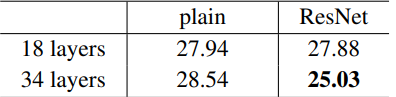
\includegraphics[width=\linewidth]{images/resnetresult1.PNG}
	\caption{Imagenet validation의Top-1 error}
 \label{fig:plainresnetresult}
	\vspace{-2mm}
\end{figure}

\newpage
\bibliography{egbib}

\end{document}
